\begin{figure}[ht]
  \centering
  %Define block styles
  \tikzstyle{decision} = [diamond, draw, fill=blue!20, 
  text width=4.5em, text badly centered, node distance=3cm, inner sep=0pt]
  \tikzstyle{block} = [rectangle, draw, fill=blue!20, text width=12em, text
  centered, rounded corners, minimum height=3em]
  \tikzstyle{line} = [draw, -latex']
  \tikzstyle{cloud} = [fill=none, node distance=3cm, minimum
  height=2em]
  
    
  \begin{tikzpicture}[node distance = 2cm, auto]
    % Place nodes
    \node[cloud] (theory) {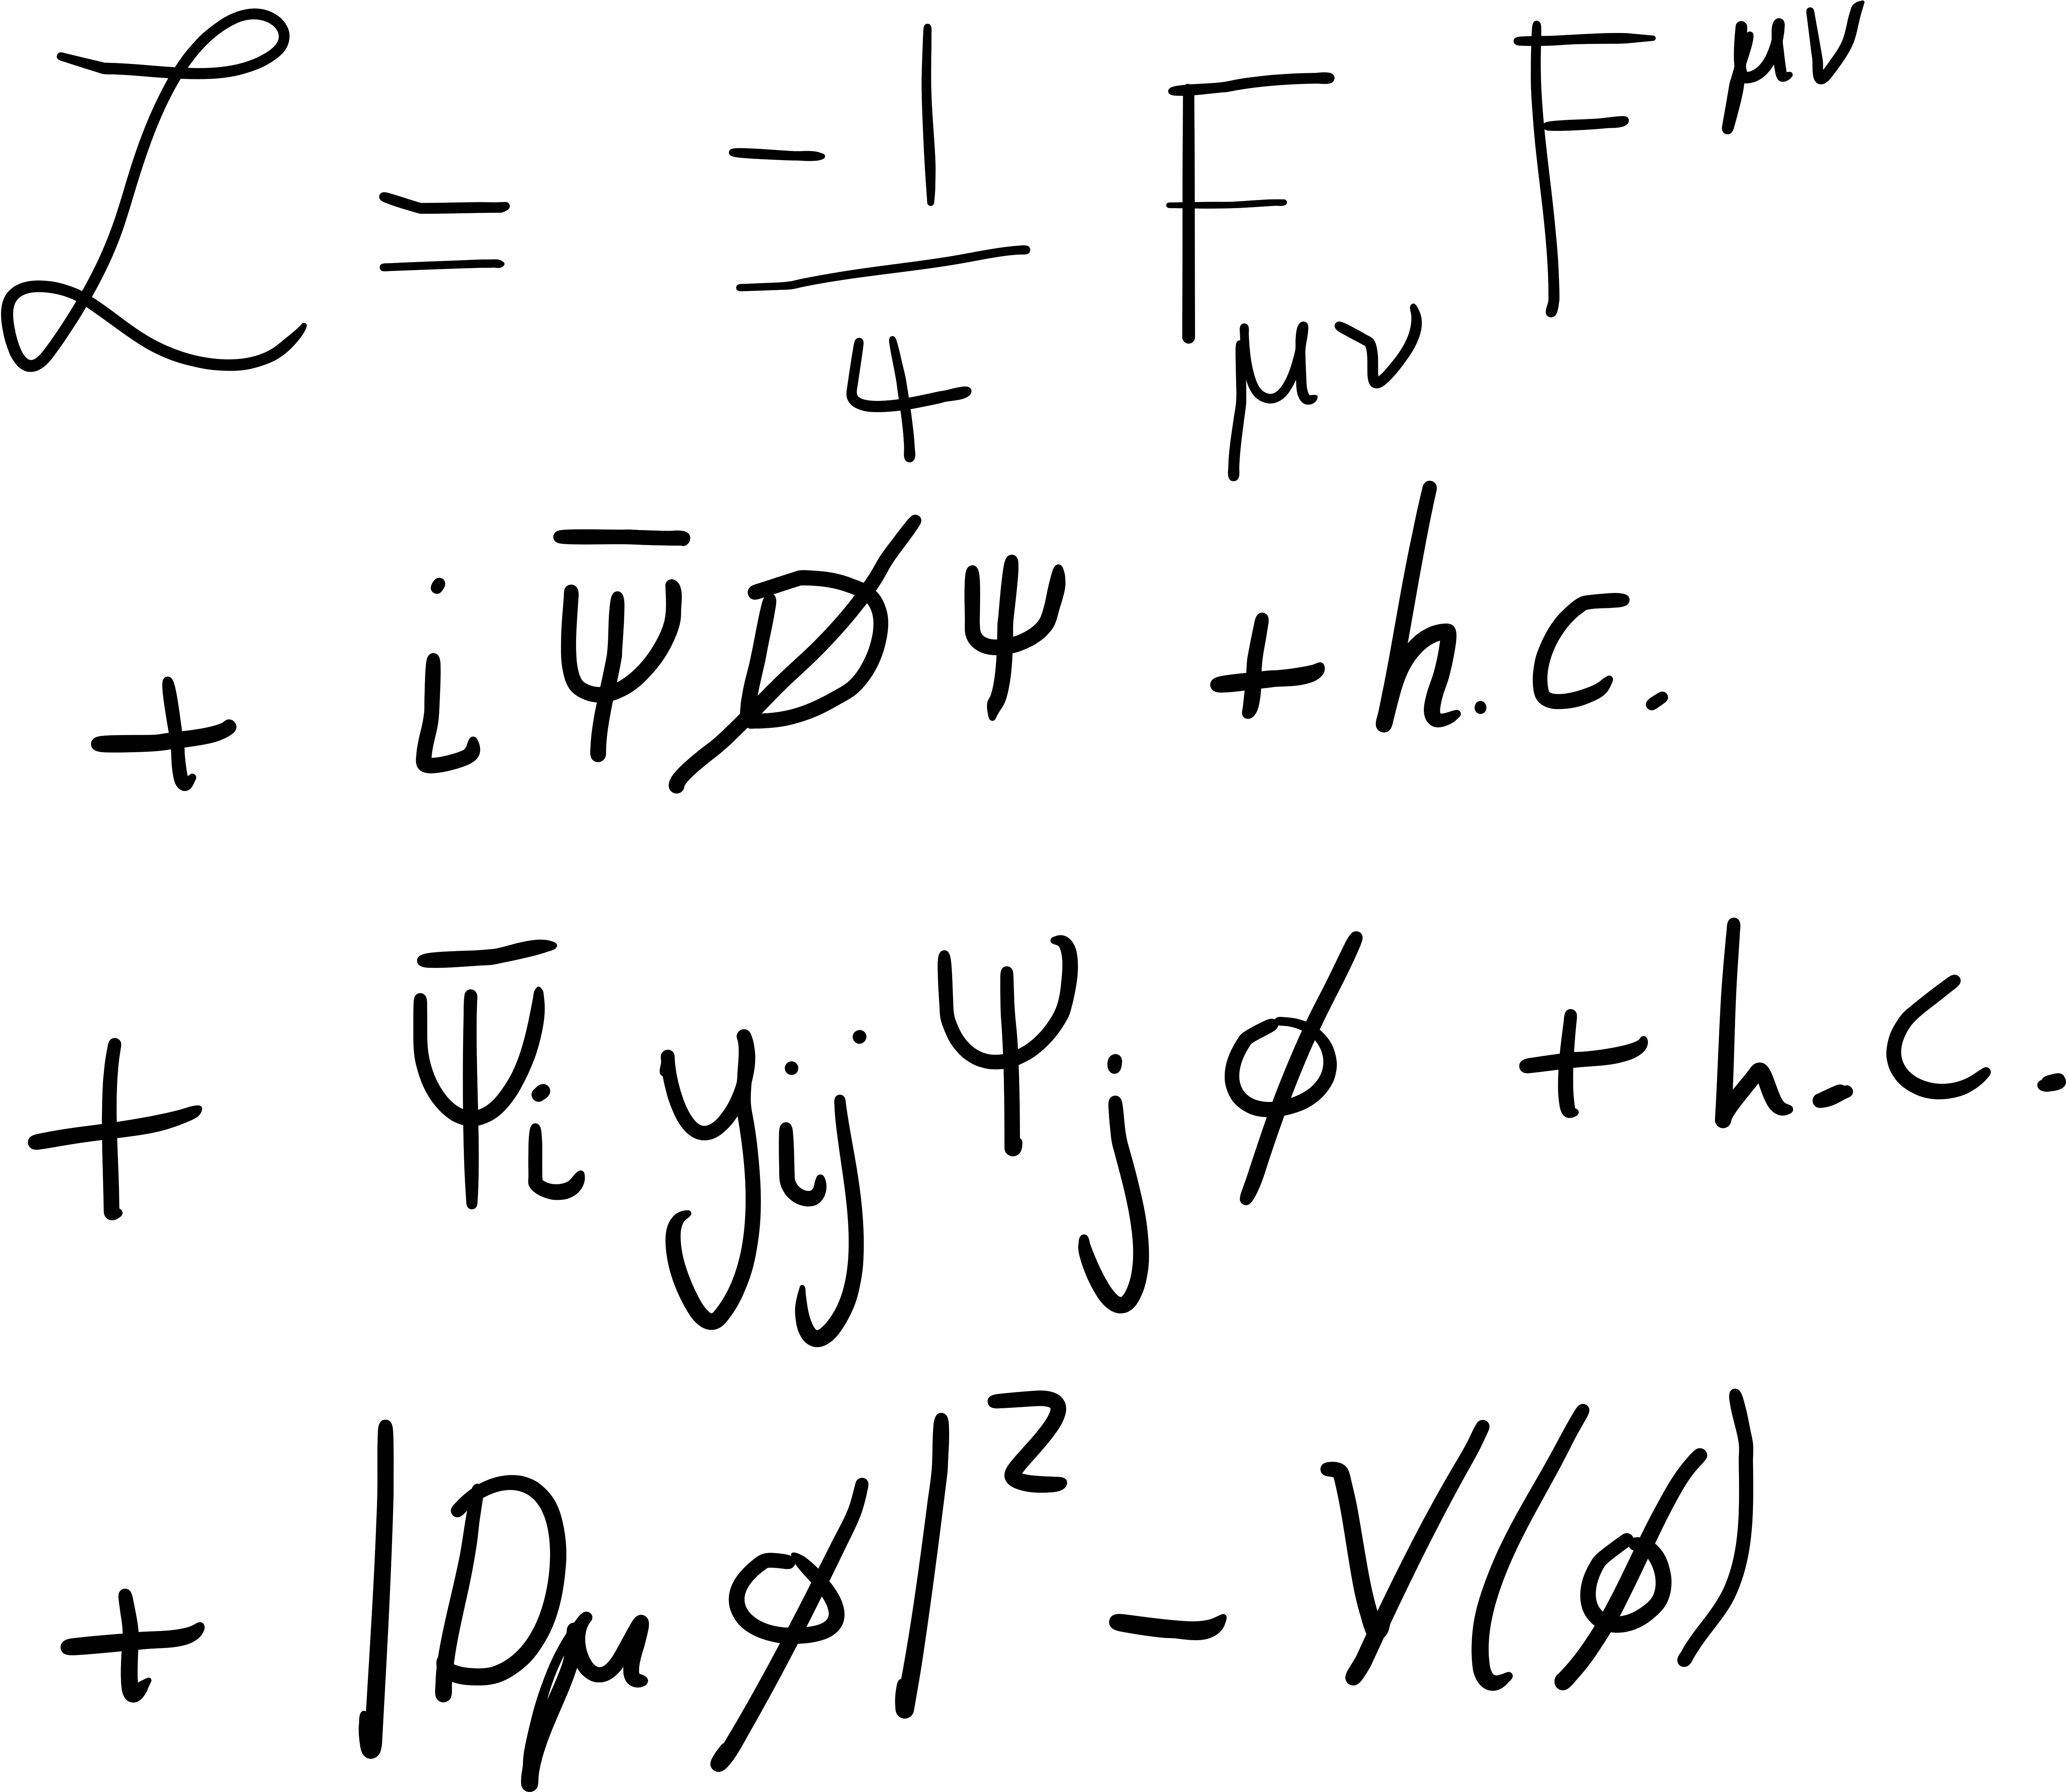
\includegraphics[width=.25\textwidth]{hand_written_lagrangian-1}};
    
    \node [cloud, right=of theory] (detector)  {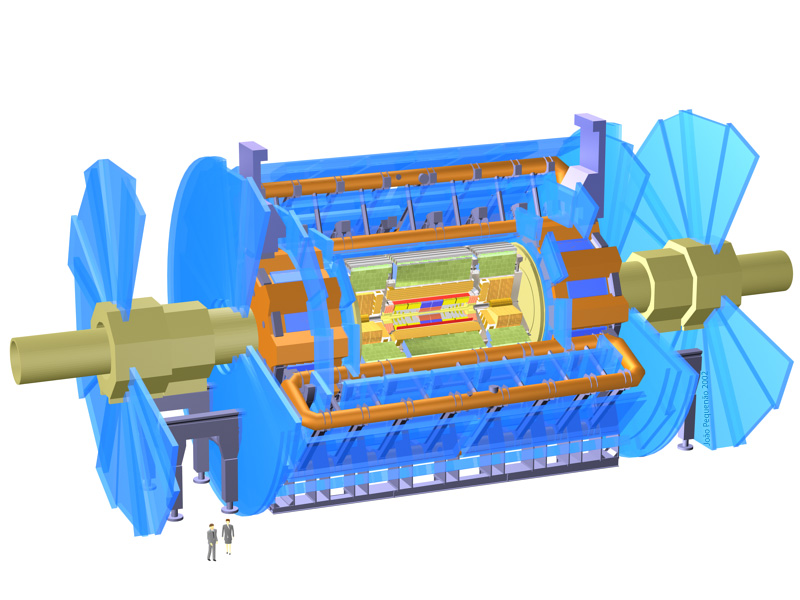
\includegraphics[width=.25\textwidth]{atlas_big}};

    \node [cloud, below left=of detector] (recon)  {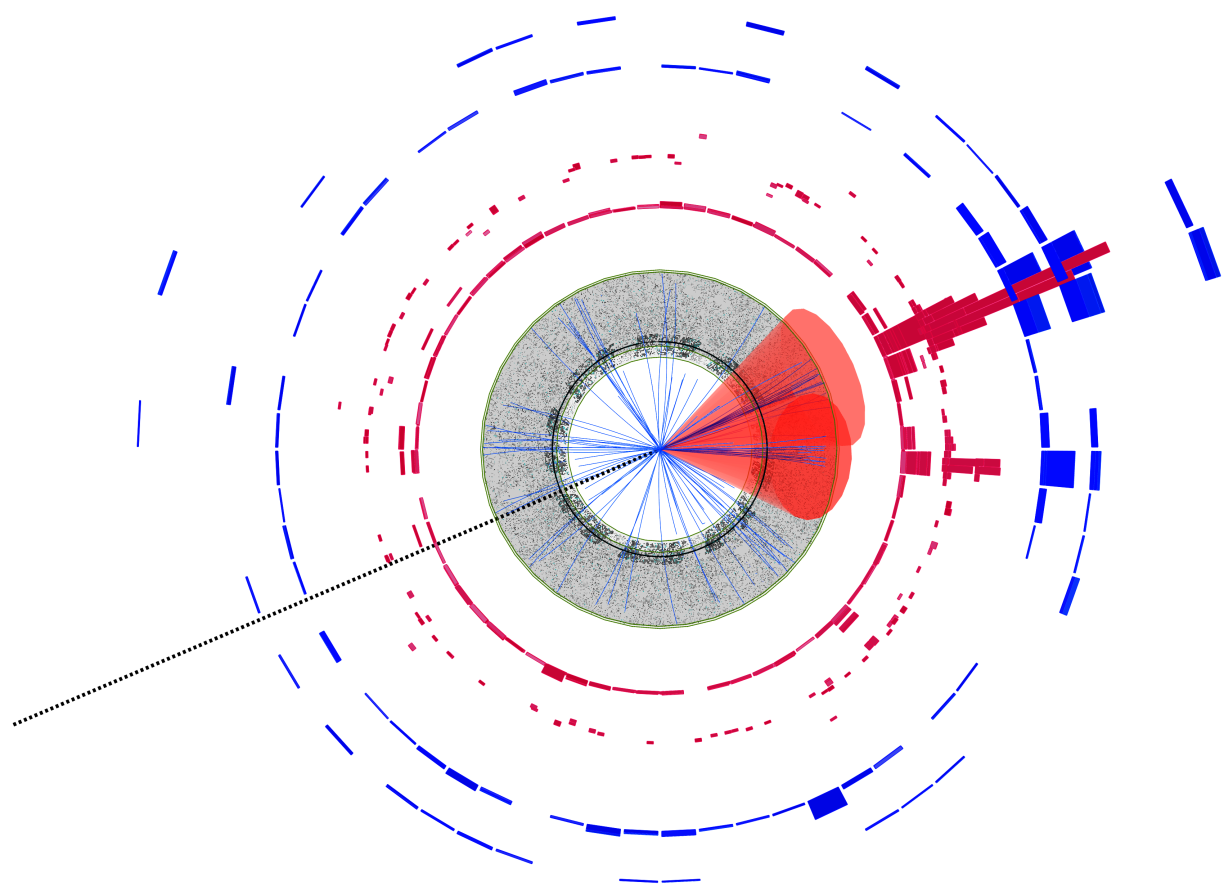
\includegraphics[width=.25\textwidth]{Event_Display_inv}};

    \node [cloud, below left=of recon] (modelling)  {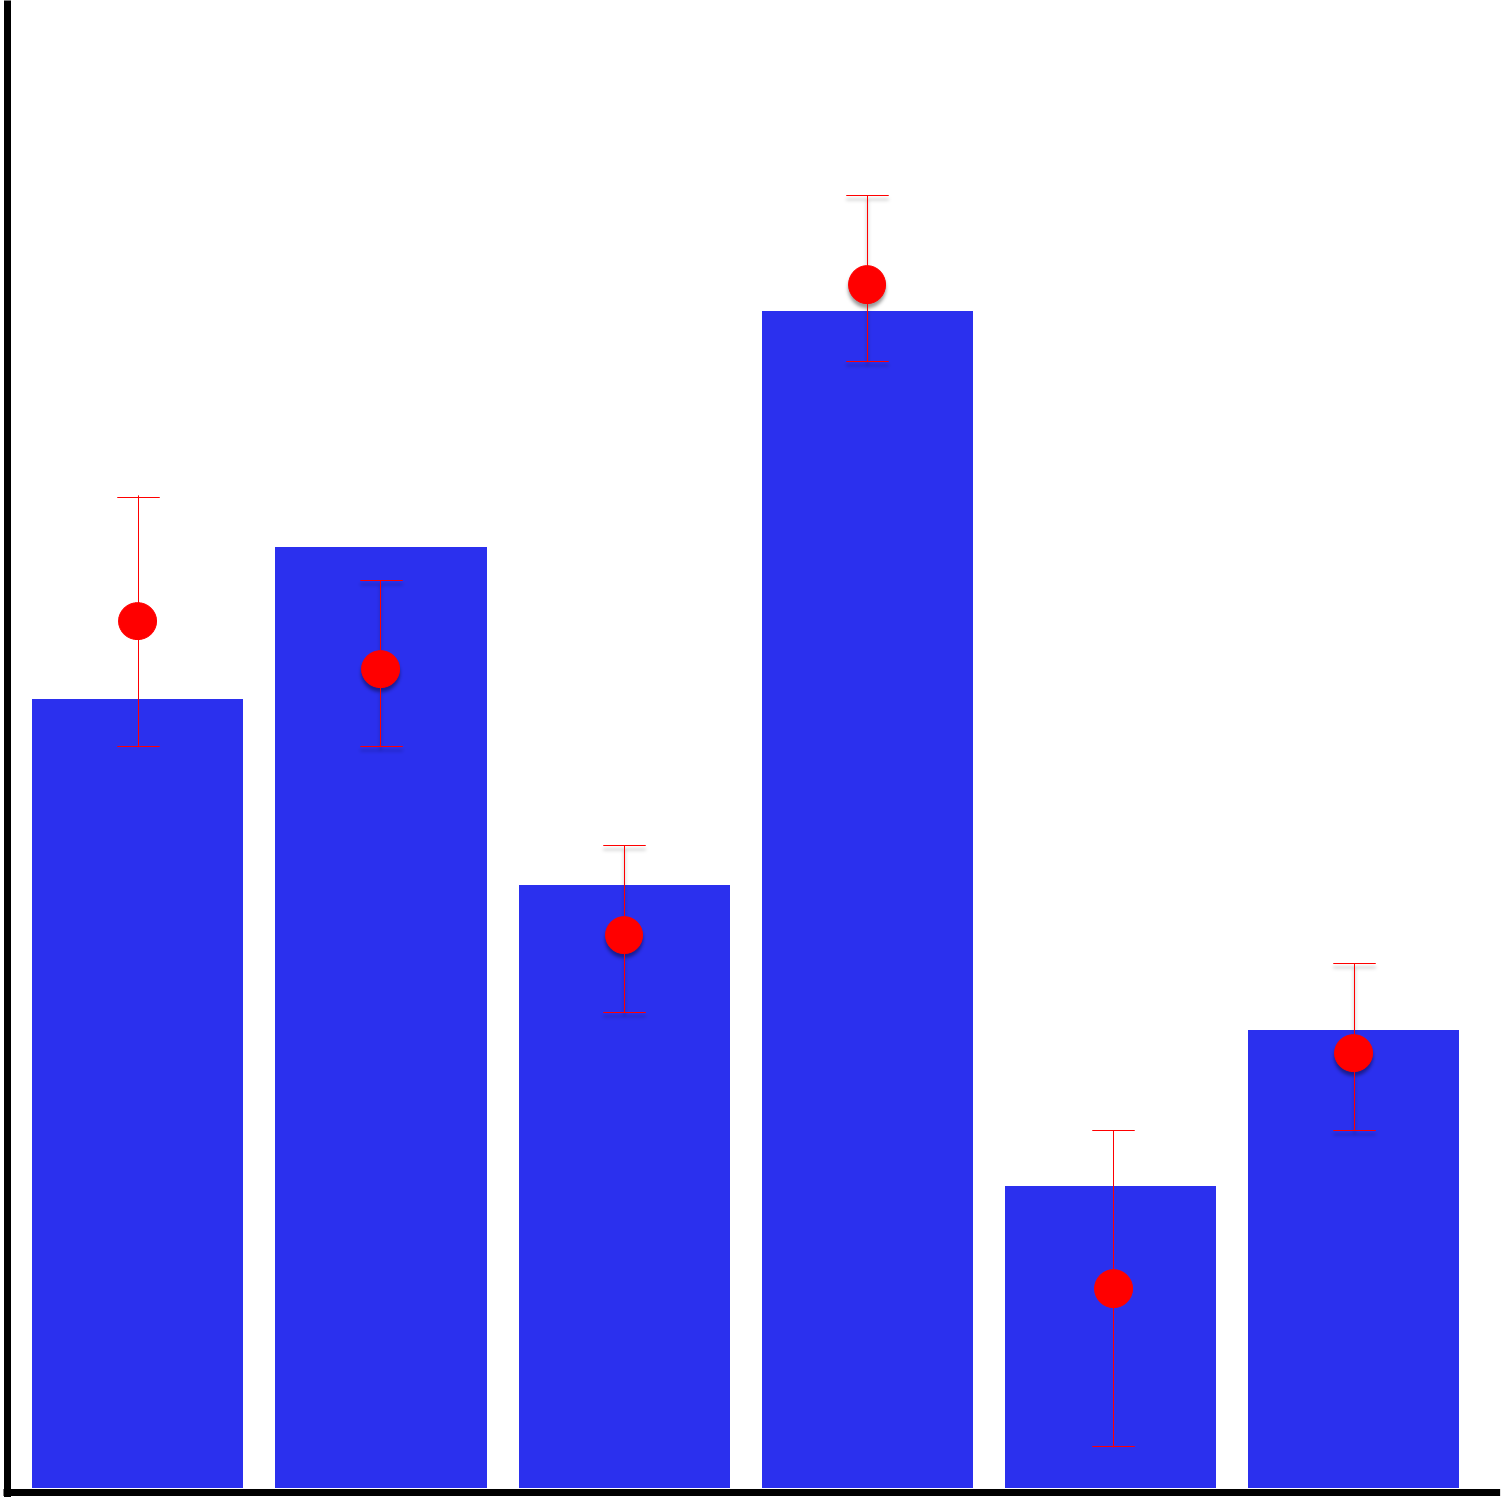
\includegraphics[width=.25\textwidth]{generic_data_mc}};

    \node [cloud, below right=of recon] (mva)  {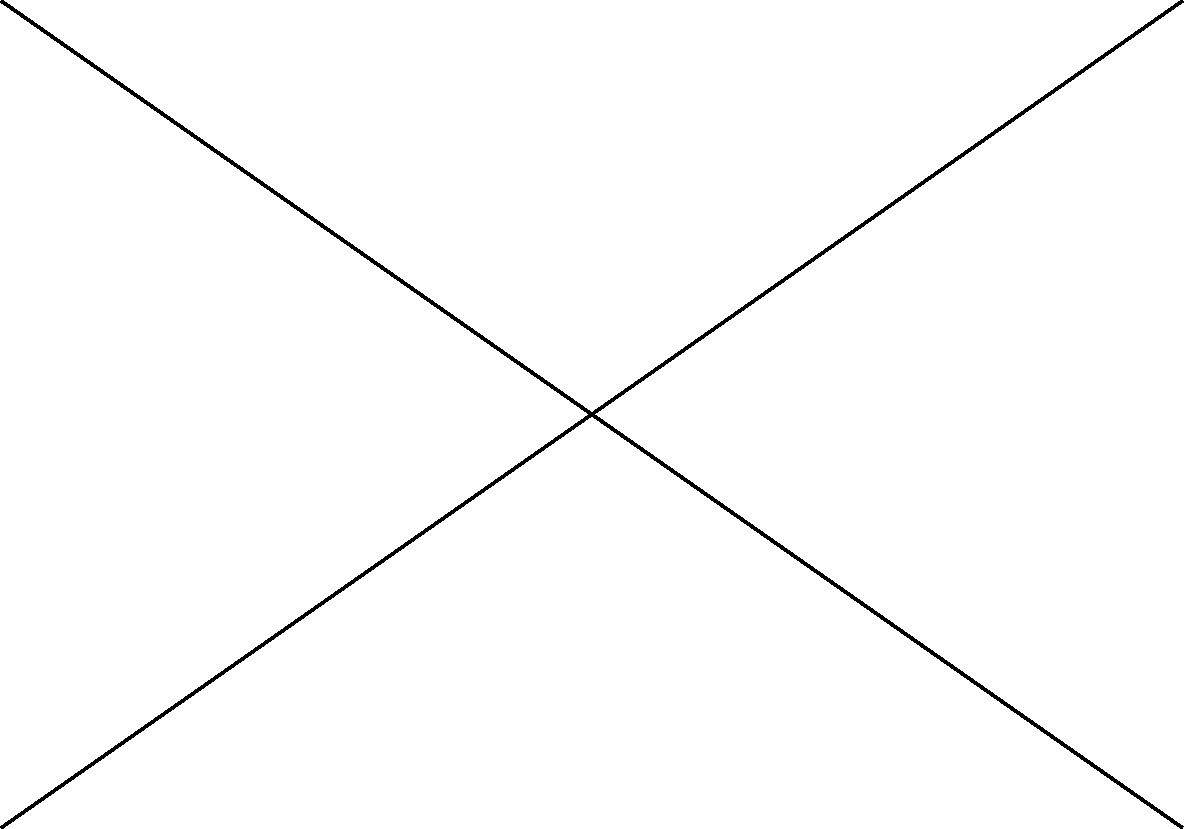
\includegraphics[width=.25\textwidth]{placeholder}};

    \node [cloud, below right=of modelling] (plf)  {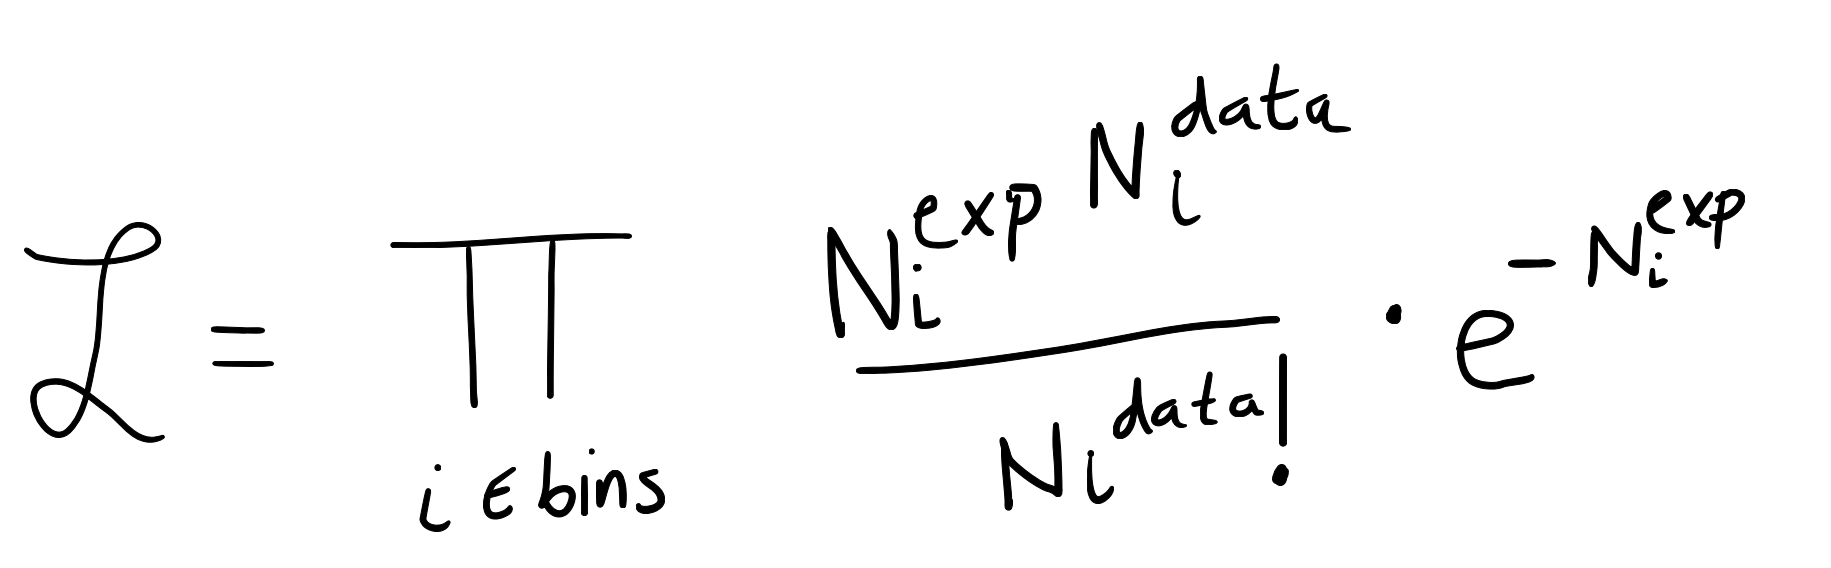
\includegraphics[width=.45\textwidth]{plf_handwritten}};

    \node [cloud, below=of plf] (results)  {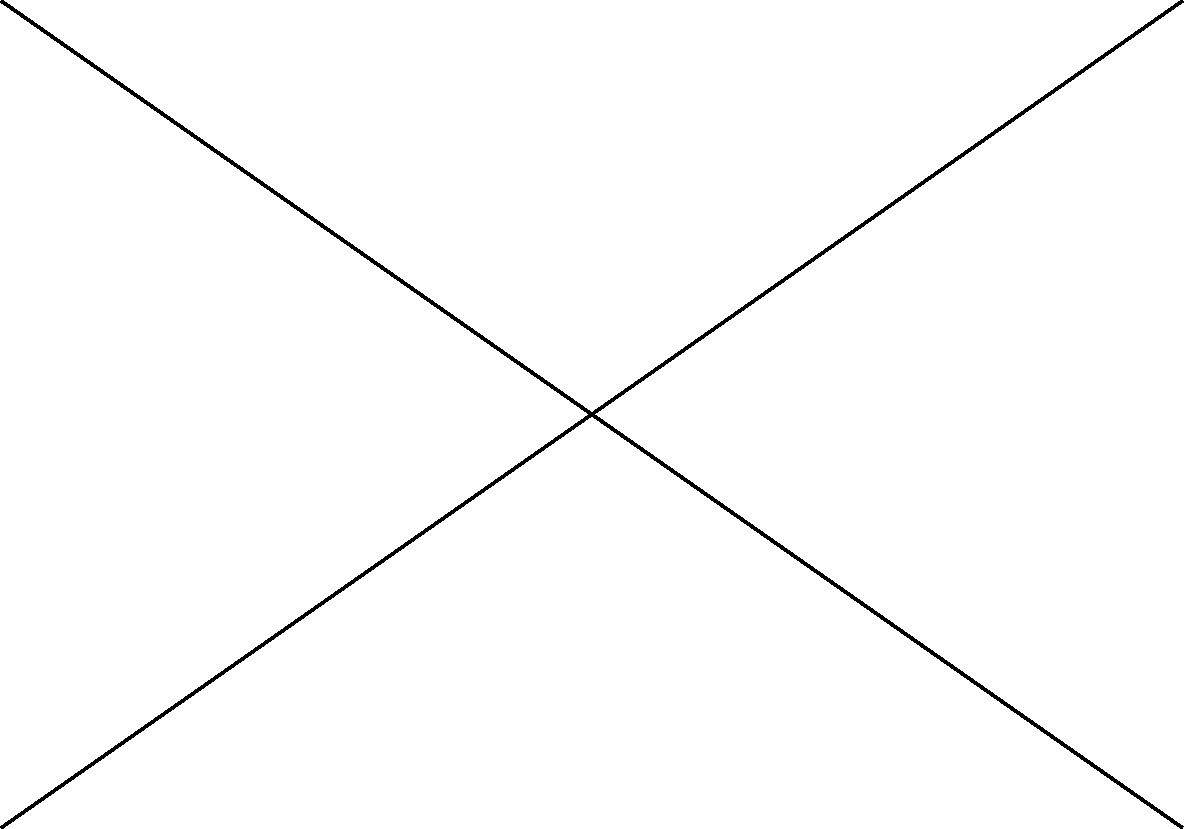
\includegraphics[width=.25\textwidth]{placeholder}};
    
    % Draw edges 
    \path [line] (theory) -- (detector);

    \path [line] (detector) -- (recon);

    \path [line] (detector) to [out=200,in=70] (modelling);

    \path [line] (recon) -- (modelling);

    \path [line] (recon) -- (mva);

    \path [line] (mva) -- (plf);

    \path [line] (modelling) -- (plf);

    \path [line] (plf) -- (results);
    
  \end{tikzpicture}
  \caption{A flow chart showing the roadmap of the VHbb analysis and of this thesis.}
  \label{fig:cxaod-flow}
\end{figure}

